\documentclass{article}
\usepackage[margin=1in]{geometry}
\usepackage{amsmath}
\usepackage{graphicx}
\usepackage{float}
\usepackage{listings}
\usepackage{xcolor}

\lstset{
    language=Matlab,
    basicstyle=\ttfamily\footnotesize,
    keywordstyle=\color{blue},
    breaklines=true
}

\begin{document}

\section*{Problem 2(b)}

The right boundary condition is changed from a Dirichlet condition ($u(1,t)=0$) to a homogeneous Neumann condition ($\frac{\partial u}{\partial x}\big|_{x=L}=0$). 

\subsection*{Finite Element Implementation}
In the finite element method, Dirichlet conditions are essential boundary conditions that must be explicitly enforced by modifying the global algebraic system (clamping the matrix row). Conversely, Neumann conditions are natural boundary conditions. Because the prescribed flux is zero, the boundary term in the weak formulation naturally vanishes. Therefore, to implement this condition, the explicit clamping of the last row of the global matrix and load vector is simply removed.

\subsection*{Results and Comparison}
Comparing the solution at $t=1.5$ to the results from part 2(a), the differences can be seen at the right boundary ($x=1$). 

In 2(a), the Dirichlet condition forced the solution to zero creating a sharp, unnatural gradient as the wave propagated to the right in the domain. In 2(b), the natural Neumann condition allows the wave to advect freely out of the domain. The value at $x=1$ is non-zero, and the spatial derivative (slope) flattens to exactly zero at the boundary, satisfying the homogeneous condition. 



\begin{figure}[H]
    \centering
    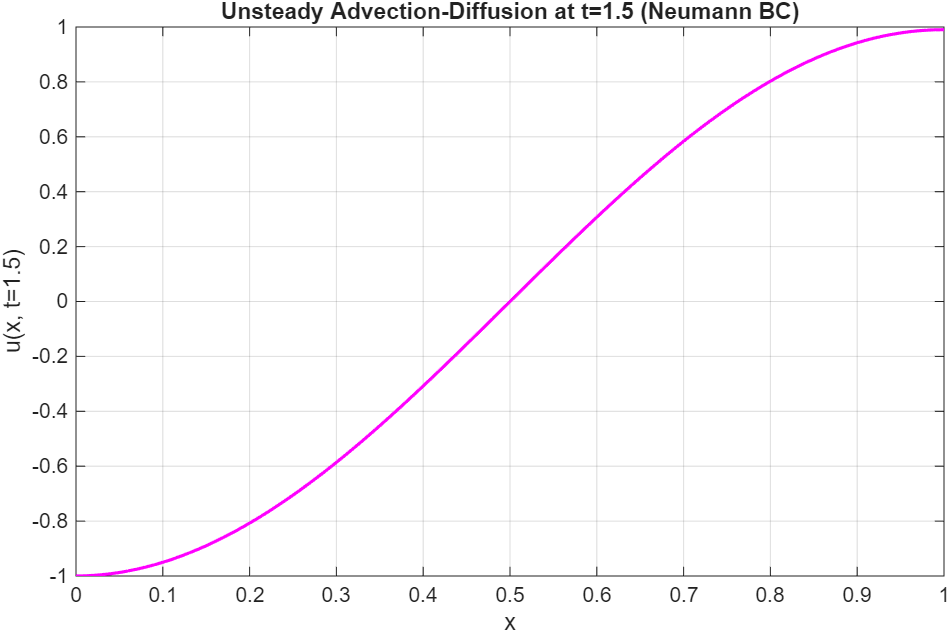
\includegraphics[width=0.7\textwidth]{2_b.png}
    \caption{Unsteady Advection-Diffusion at $t=1.5$ with a Neumann right boundary condition.}
    \label{fig:2b}
\end{figure}

\subsection*{MATLAB Implementation}
\begin{lstlisting}
L = 1.0; c = 1.0; nu = 1e-3; f = 0.0;
E = 100; N = E + 1; h = L / E;
dt = 0.001; t_end = 1.5;
n_steps = round(t_end / dt);

x = linspace(0, L, N)';
A = sparse(N, N); C = sparse(N, N); B = sparse(N, N);

for e = 1:E
    A_e = (1.0 / h) * [1.0, -1.0; -1.0, 1.0];
    C_e = 0.5 * [-1.0, 1.0; -1.0, 1.0];
    B_e = (h / 6.0) * [2.0, 1.0; 1.0, 2.0];
    
    idx = [e, e+1];
    A(idx, idx) = A(idx, idx) + A_e;
    C(idx, idx) = C(idx, idx) + C_e;
    B(idx, idx) = B(idx, idx) + B_e;
end

U = zeros(N, n_steps + 1);

LHS1 = (1/dt)*B + nu*A;
LHS2 = (3/(2*dt))*B + nu*A;
LHS3 = (11/(6*dt))*B + nu*A;

for n = 1:n_steps
    t_next = n * dt;
    
    if n == 1
        RHS = (1/dt)*B*U(:, n) - c*C*U(:, n);
        LHS = LHS1;
    elseif n == 2
        RHS = (1/dt)*B*(2*U(:, n) - 0.5*U(:, n-1)) - c*C*(2*U(:, n) - U(:, n-1));
        LHS = LHS2;
    else
        RHS = (1/dt)*B*(3*U(:, n) - 1.5*U(:, n-1) + (1/3)*U(:, n-2)) - ...
              c*C*(3*U(:, n) - 3*U(:, n-1) + U(:, n-2));
        LHS = LHS3;
    end
    
    LHS_bc = LHS;
    
    LHS_bc(1, :) = 0; 
    LHS_bc(1, 1) = 1; 
    RHS(1) = sin(pi * t_next);
    
    U(:, n+1) = LHS_bc \ RHS;
end
\end{lstlisting}

\end{document}